{Proving that given equation represents two straight lines}
The given equation is
\begin{align}\label{eq:solutions/13/2/eq:e1}
    x^2-5xy+4y^2+x+2y-2=0
\end{align}
Comparing this to the standard equation,
\begin{align}
    \vec{V} = \myvec{1 & \frac{-5}{2} \\ \frac{-5}{2} & 4}\\
    \vec{u} = \myvec{\frac{1}{2} \\ 1}\\
    f = -2
\end{align}
\begin{align}\label{eq:solutions/13/2/eq:e3}
    \implies\vec{x}^T\myvec{1 & \frac{-5}{2} \\ \frac{-5}{2} & 4}\vec{x} + 2\myvec{\frac{1}{2} & 1}\vec{x} -2 = 0
\end{align}
Equation \eqref{eq:solutions/13/2/eq:e1} represents a pair of straight lines if
\begin{align}
    \label{eq:solutions/13/2/eq:det}\mydet{\vec{V} & \vec{u}\\ \vec{u}^T & f}=0
\end{align}
\begin{align}
    \delta & = \mydet{1 & \dfrac{-5}{2} & \dfrac{1}{2} \\ \dfrac{-5}{2} & 4 & 1 \\ \dfrac{1}{2} & 1 & -2} \\ & = 0
\end{align}
Hence, proved that given equation represents two straight lines.
{Finding point of intersection between the straight lines}
\begin{align}
    \det V & = \mydet{1 & \frac{-5}{2}\\ \frac{-5}{2} & 4}\\ & = \frac{-9}{4} < 0
\end{align}
Thus, the two straight lines intersect. Let the equation of the straight lines be given as
\begin{align}
    \label{eq:solutions/13/2/eq:line1}\vec{n}_1^T\vec{x}=c_1 \\
    \label{eq:solutions/13/2/eq:line2}\vec{n}_2^T\vec{x}=c_2
\end{align}
with their slopes as $\vec{m}_1$ and $\vec{m}_2$ respectively.

Then the equation of the pair of straight lines is
\begin{align}\label{eq:solutions/13/2/eq:line1line2}
    (\vec{n}_1^T\vec{x}-c_1)(\vec{n}_2^T\vec{x}-c_2) = 0
\end{align}
Using \eqref{eq:solutions/13/2/eq:e3} and \eqref{eq:solutions/13/2/eq:line1line2},
\begin{align}
    (\vec{n}_1^T\vec{x}-c_1)(\vec{n}_2^T\vec{x}-c_2) = \vec{x}^T\myvec{1 & \frac{-5}{2} \\ \frac{-5}{2} & 4}\vec{x} + 2\myvec{\frac{1}{2} & 1}\vec{x} -2
\end{align}
Comparing both sides,
\begin{align}
    c_2\vec{n}_1+c_1\vec{n}_2 = -2\myvec{\frac{1}{2} \\ 1}\label{eq:solutions/13/2/eq:c1c2}\\
    c_1c_2 = -2
\end{align}
Slopes of the lines are roots of the equation
\begin{align}
    cm^2+2bm+a=0 \label{eq:solutions/13/2/eq:slope}\\
    \implies m_i = \frac{-b\pm \sqrt{-\mydet{\vec{V}}}}{c}\\
    \vec{n}_i = k_i\myvec{-m_i \\ 1}
\end{align}
Substituting \eqref{eq:solutions/13/2/eq:e1} in \eqref{eq:solutions/13/2/eq:slope},
\begin{align}
    4m^2-5m+1=0\\
    \implies m_i = \frac{\frac{5}{2}\pm \frac{3}{2}}{4} \\
    \implies m_1 = 1, m_2 = \frac{1}{4}
\end{align}
Therefore,
\begin{align}
    \vec{n}_1=k_1\myvec{-1 \\ 1}\\
    \vec{n}_2=k_2\myvec{\frac{-1}{4} \\ 1}
\end{align}
We know that
\begin{align}
	\label{eq:solutions/13/2/n1n2}\vec{n}_1*\vec{n}_2 = \myvec{a\\2b\\c}\\
	k_1\myvec{-1 \\ 1}*k_2\myvec{\frac{-1}{4} \\ 1} = \myvec{1 \\ -5 \\ 4}\\
	\implies k_1k_2 = 4
\end{align}
Taking $k_1 = 1$, $k_2 = 4$, we get
\begin{align}
    \vec{n}_1 = \myvec{-1 \\ 1}\nonumber\\
    \vec{n}_2 = \myvec{-1 \\ 4}\label{eq:solutions/13/2/eq:nvalues}
\end{align}
For verifying values of $\vec{n}_1$ and $\vec{n}_2$, we compute the convolution by representing $\vec{n}_1$ as Toeplitz matrix,
\begin{align}
    \vec{n}_1*\vec{n}_2=\myvec{-1 & 0 \\ 1 & -1 \\ 0 & 1}\myvec{-1 \\ 4} = \myvec{1 \\ -5 \\ 4}
\end{align}
Now, obtaining $c_1$ and $c_2$ using \eqref{eq:solutions/13/2/eq:nvalues} and \eqref{eq:solutions/13/2/eq:c1c2}
\begin{align}
    \myvec{\vec{n}_1 & \vec{n}_2}\myvec{c_2 \\ c_1} = -2\myvec{\frac{1}{2} \\ 1}\\
    \implies \myvec{-1 & -1 \\ 1 & 4}\myvec{c_2 \\ c_1} = \myvec{-1 \\ -2}
\end{align}
Row reducing the augmented matrix,
\begin{align}
    \myvec{-1 & -1 & -1 \\ 1 & 4 & -2} \xleftrightarrow{R_1 \leftarrow -R_1}\myvec{1 & 1 & 1 \\ 1 & 4 & -2}\\\xleftrightarrow{R_2\leftarrow R_2-R_1}\myvec{1 & 1 & 1 \\ 0 & 3 & -3}\\
    \xleftrightarrow{R_1\leftarrow R_1-R_2}\myvec{1 & 0 & 2 \\ 0 & 1 & -1}
\end{align}
\begin{align}
    \implies \myvec{1 & 0 \\ 0 & 1}\myvec{c_2 \\ c_1} = \myvec{2 \\ -1}\nonumber\\
    c_1 = -1\\
    c_2 = 2\label{eq:solutions/13/2/eq:cvalues}
\end{align}
Thus, equation of lines can be written as
\begin{align}
    \myvec{-1 & 1}\vec{x} = -1\\
    \myvec{-1 & 4}\vec{x} = 2
\end{align}
Augmented matrix for these set of equations is
\begin{align}
    \myvec{-1 & 1 & -1 \\ -1 & 4 & 2}\xleftrightarrow{R_1\leftarrow -R_1}\myvec{1 & -1 & 1 \\ -1 & 4 & 2}\\\xleftrightarrow{R_2\leftarrow R_2+R_1}\myvec{1 & -1 & 1 \\ 0 & 3 & 3}
    \xleftrightarrow{R_2\leftarrow \frac{R_2}{3}}\myvec{1 & -1 & 1 \\ 0 & 1 & 1}\\\xleftrightarrow{R_1\leftarrow R_1+R_2}\myvec{1 & 0 & 2 \\ 0 & 1 & 1}
\end{align}
Thus, the point of intersection is $\vec{A} = \myvec{2 \\ 1}$.
\begin{figure}[h!]
    \centering
    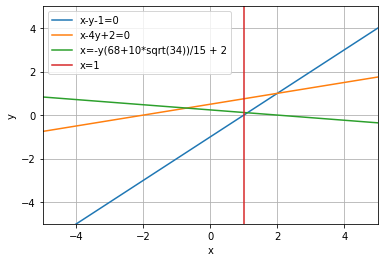
\includegraphics[width=\columnwidth]{./solutions/13/2/assignment3.png}
    \caption{Intersection of pair of original pair of straight lines and the pair of straight lines after affine transform}
    \label{eq:solutions/13/2/fig:fig1}
\end{figure}

Using \eqref{eq:solutions/13/2/eq:nvalues} and \eqref{eq:solutions/13/2/eq:cvalues} in \eqref{eq:solutions/13/2/eq:line1line2}, equation of the pair of straight lines is
\begin{align}
    (x-y-1)(x-4y+2) = 0
\end{align}

{Angle between lines}
Angle between pair of lines is,
\begin{align}\label{eq:solutions/13/2/eq:cos}
    \theta = \cos^{-1}\left(\frac{\vec{n}_1^T\vec{n}_2}{\norm{\vec{n}_1}\norm{\vec{n}_2}}\right)
\end{align}
\begin{align}
    \vec{n}_1^T\vec{n}_2 = \myvec{-1 & 1}\myvec{-1 \\ 4} = 5 \label{eq:solutions/13/2/eq:a2} 
\end{align}
\begin{align}
    \norm{\vec{n}_1}=\sqrt{(-1)^2+1^2}=\sqrt{2}\\
    \norm{\vec{n}_2}=\sqrt{(-1)^2+4^2}=\sqrt{17} \label{eq:solutions/13/2/eq:}
\end{align}
Substituting these values \eqref{eq:solutions/13/2/eq:cos}
\begin{align}
    \theta = 30.9\degree
\end{align}
Hence, angle between the given pair of straight lines is $30.9\degree$
{Affine Transformation and Eigen Value decomposition}
First, verifying if $\vec{u}^T\vec{V}^{-1}\vec{u}-f = 0$. To do this, finding $V^{-1}$ by augmenting with identity matrix and row reducing as follows :
\begin{align}
    \myvec{1 & \frac{-5}{2} & 1 & 0\\ \frac{-5}{2} & 4 & 0 & 1}\xleftrightarrow{R_2\leftarrow R_2 + \frac{5}{2}R_1}\myvec{1 & \frac{-5}{2} & 1 & 0\\ 0 & \frac{-9}{4} & \frac{5}{2} & 1}\\\xleftrightarrow{R_2\leftarrow\frac{-4}{9}R_2}\myvec{1 & \frac{-5}{2} & 1 & 0\\ 0 & 1 & \frac{-10}{9} & \frac{-4}{9}}\\\xleftrightarrow{R_1\leftarrow R_1 + \frac{5}{2}R_2}\myvec{1 & 0 & \frac{-16}{9} & \frac{-10}{9}\\ 0 & 1 & \frac{-10}{9} & \frac{-4}{9}}\\
    \implies\vec{V}^{-1} = \myvec{\frac{-16}{9} & \frac{-10}{9} \\ \frac{-10}{9} & \frac{-4}{9}}
\end{align}
\begin{align}
    u^TV^{-1}u-f & = \myvec{\frac{1}{2} & 1}\myvec{\frac{-16}{9} & \frac{-10}{9} \\ \frac{-10}{9} & \frac{-4}{9}}\myvec{\frac{1}{2} \\ 1} - (-2) \\ & = 0
\end{align}
The characteristic equation of $\vec{V}$ is given as :
\begin{align}
    \mydet{\lambda\vec{I}-\vec{V}} = \mydet{\lambda - 1 & \frac{5}{2} \\ \frac{5}{2} & \lambda - 4} = 0\\
    \implies (\lambda - 1)(\lambda - 4) - \dfrac{25}{4} = 0\\
    \label{eq:solutions/13/2/eq:characteristic}\implies 4\lambda^2-20\lambda-9 = 0
\end{align}
The roots of \eqref{eq:solutions/13/2/eq:characteristic}, i.e. the eigenvalues of $\vec{V}$ are
\begin{align}
    \lambda_1 = \dfrac{5+\sqrt{34}}{2}, \lambda_2 = \dfrac{5-\sqrt{34}}{2}\label{eq:solutions/13/2/eq:eigenval}
\end{align}
The eigen vector $\vec{p}$ is defined as, 
\begin{align}
    \vec{V}\vec{p} &= \lambda\vec{p}\\
    \implies(\lambda\vec{I}-\vec{V})\vec{p}=0
\end{align}
For $\lambda_1=\dfrac{5+\sqrt{34}}{2}$
\begin{align}
    (\lambda_1\vec{I}-\vec{V}) = \myvec{\frac{3+\sqrt{34}}{2} & \frac{5}{2} \\ \frac{5}{2} & \frac{-3 +\sqrt{34}}{2}}
\end{align}
To find $\vec{p}_1$, let's look at Augmented form of $(\lambda_1\vec{I}-\vec{V})$
\begin{align}
    \myvec{\frac{3+\sqrt{34}}{2} & \frac{5}{2} & 0 \\ \frac{5}{2} & \frac{-3 +\sqrt{34}}{2} & 0}\\\xleftrightarrow{R_1 \leftarrow \frac{2}{3+\sqrt{34}}R_1}\myvec{1 & \frac{-3+\sqrt{34}}{5} & 0 \\ \frac{5}{2} & \frac{-3 +\sqrt{34}}{2} & 0}\\\xleftrightarrow{R_2\leftarrow \frac{2}{5}R_2 - R_1}\myvec{1 & \frac{-3+\sqrt{34}}{5} & 0 \\ 0&0&0}
\end{align}
So we get
\begin{align}
    x_1 + \left(\frac{-3+\sqrt{34}}{5}\right) x_2 = 0
\end{align}
Thus, our eigenvector corresponding to $\lambda_1$
\begin{align}
    \vec{p}_1 = \myvec{\frac{3-\sqrt{34}}{5} \\ 1}
\end{align}
For $\lambda_2=\dfrac{5-\sqrt{34}}{2}$
\begin{align}
    (\lambda_2\vec{I}-\vec{V}) = \myvec{\frac{3-\sqrt{34}}{2} & \frac{5}{2} \\ \frac{5}{2} & \frac{-3 -\sqrt{34}}{2}}
\end{align}
To find $\vec{p}_2$, let's look at Augmented form of $(\lambda_2\vec{I}-\vec{V})$
\begin{align}
    \myvec{\frac{3-\sqrt{34}}{2} & \frac{5}{2} & 0 \\ \frac{5}{2} & \frac{-3 -\sqrt{34}}{2} & 0}\\\xleftrightarrow{R_1 \leftarrow \frac{2}{3-\sqrt{34}}R_1}\myvec{1 & \frac{-3-\sqrt{34}}{5} & 0 \\ \frac{5}{2} & \frac{-3 -\sqrt{34}}{2} & 0}\\\xleftrightarrow{R_2\leftarrow \frac{2}{5}R_2 - R_1}\myvec{1 & \frac{-3-\sqrt{34}}{5} & 0 \\ 0&0&0}
\end{align}
So we get
\begin{align}
    x_1 + \left(\frac{-3-\sqrt{34}}{5}\right) x_2 = 0
\end{align}
Thus, our eigenvector corresponding to $\lambda_2$
\begin{align}
    \vec{p}_2 = \myvec{\frac{3+\sqrt{34}}{5} \\ 1}
\end{align}
We know $\vec{V} = \vec{P}\vec{D}\vec{P}^{T}$, where $\vec{P}$ and the diagonal matrix $\vec{D}$ are given as:
\begin{align}
    \vec{D} & = \myvec{\lambda_1 & 0 \\ 0 & \lambda_2}\\ & = \myvec{\frac{5+\sqrt{34}}{2} & 0\\ 0 & \frac{5-\sqrt{34}}{2}}\label{eq:solutions/13/2/eq:DVal}\\
    \vec{P} & = \myvec{\vec{p}_1 & \vec{p}_2}\\&= \myvec{\frac{3-\sqrt{34}}{5} & \frac{3+\sqrt{34}}{5}\\ 1 & 1}\label{eq:solutions/13/2/eq:PVal}
\end{align}
So, the equation of the pair of straight lines is given by :
\begin{align}
    \vec{y}^T\vec{D}\vec{y} = \vec{u}^T\vec{V}^{-1}\vec{u}-f\qquad\text{$\mydet{\vec{V}}\neq0$}\\
    \vec{y}^T\myvec{\dfrac{5+\sqrt{34}}{2} & 0\\ 0 & \dfrac{5-\sqrt{34}}{2}}\vec{y} =0\\
    \implies \myvec{y_1 & y_2}\myvec{\dfrac{5+\sqrt{34}}{2} & 0\\ 0 & \dfrac{5-\sqrt{34}}{2}}\myvec{y_1 \\ y_2} = 0\\
    \implies (5+\sqrt{34})y_1^2 + (5-\sqrt{34})y_2^2 = 0
\end{align}
So we get the equation of the pair of straight lines, as we can see this passes through the origin $(0,0)$. The corresponding image is shown in Fig. \ref{eq:solutions/13/2/fig:fig2}
\begin{align}
    \vec{c} = -\vec{V}^{-1}\vec{u}\qquad\text{$\mydet{\vec{V}}\neq0$}\\
    \implies \vec{c} = -\myvec{\frac{-16}{9} & \frac{-10}{9} \\ \frac{-10}{9} & \frac{-4}{9}}\myvec{\frac{1}{2} \\ 1} = \myvec{2 \\ 1}\\
    \intertext{And,}
    \vec{P}^T = \myvec{\frac{3-\sqrt{34}}{5} & 1\\ \frac{3+\sqrt{34}}{5} & 1}
    \intertext{Using affine transformation, we can express the equation as}
    \vec{x} = \vec{P}\vec{y} + \vec{c}\\
    \implies \vec{x} = \myvec{\frac{3-\sqrt{34}}{5} & \frac{3+\sqrt{34}}{5}\\1 & 1}\vec{y} + \myvec{2 \\ 1}
\end{align}
The corresponding image is shown in Fig. \ref{eq:solutions/13/2/fig:fig1}
\begin{figure}[h!]
    \centering
    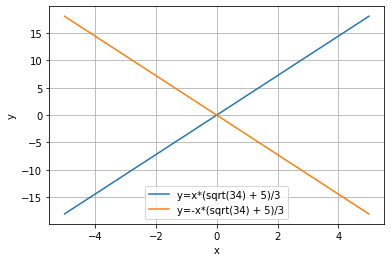
\includegraphics[width=\columnwidth]{./solutions/13/2/assignment3.1.png}
    \caption{Pair of straight lines passing through origin after eigenvalue decomposition}
    \label{eq:solutions/13/2/fig:fig2}
\end{figure}
